%%% chapter of SNO+ detector
%\setlength{\epigraphwidth}{0.5\textwidth}
%\epigraph{In all experimental science the techniques for obtaining measurements are almost as important as the measurements themselves.}{--- \textup{J. D. Bernal}, \textit{The Social Function of Science}}

\section{Overview}\label{sect:overview}
The SNO+ experiment is located at SNOLAB. This deep underground facility sits at Vale's Creighton mine in Sudbury, Ontario, Canada (coordinate: 46$^\circ$28'19.6"N, 81$^\circ$11'12.4"W). It provides an environment with extremely low cosmic ray backgrounds. At sea level, an average cosmic muon ($\mu$) flux rate is about $1.44\times 10^7~\mu/m^2/day$\cite{muonflux}. Cosmic muons with high energies (mostly $\mathcal{O}$(GeV)) can induce spallation backgrounds, such as fast neutrons and lasting isotopes, which are harmful to the low background counting experiments\cite{beacom2017physics}. The SNOLAB has a $2092\pm6$ m flat overburden of rock, which is $5890\pm94$ water equivalent meter (m.w.e). This rock overburden ensures that cosmic muon ($\mu$) flux rate is as low as $0.286\pm0.009~\mu/m^2/day$\cite{snop_jinst}, which means that every hour only about 1 $\mu$ passes through the SNO+ detector. 

The SNO+ detector is a refurbishment of the SNO detector. The SNO+ collaboration makes use of the SNO infrastructure and upgraded it to be a liquid scintillator detector. As shown in Fig.~\ref{snopdetector}, the detector is inside a barrel-like rock cavity with a diameter of 22 m at its waist and a height of 34 m. The cavity is filled with 7000 tonnes of ultrapure water (UPW) to provide buoyancy for the vessel, and shield radiation backgrounds from the environment, such as the cosmic rays and isotope decays from the rock. 

The detector consists of an acrylic vessel (AV) sphere of 12.01 m in diameter and 5.5 cm in thickness. The AV contains detection media (or called target materials) and is held in place by a rope net system including hold-up and hold-down Tensylon ropes. This spherical structure is simple in geometry and reduces the complexities of simulation and event reconstruction. Furthermore, this geometry allows for spherical fiducial volume cuts from the center of the AV to further get rid of external backgrounds, which makes the SNO+ as a graded-shield type detector\cite{waterfield2017optical}.
On the top of the AV sphere, there is an acrylic neck cylinder with 6.8 m high and 1.46 m inner diameter. The neck connects the AV sphere to the facilities on the deck above the detector. Through the neck, pipes can fill the detection media into the AV and recirculate as well. Calibration sources for internal scans can also be lowered down into the AV through the neck.

The AV sphere is concentric within a stainless steel geodesic dome with an average radius of 8.4 m, which is called the photomultiplier support structure (PSUP). 9394 Hamamatsu 8-inch R1408 photomultipliers (PMTs) were mounted on the PSUP, looking inward to the AV. To increase the light collection efficiency of these PMTs and thus to obtain an extensive photocathode coverage of the detector, each of these PMTs was fitted into a 27 cm diameter reflective bucket (called ``concentrator''), which consists of reflective pedals coated with aluminum. The effective photocathode coverage of the detector reaches about 54\%\cite{whitepaper}. Besides the inward-looking PMTs, 90 PMTs look outward, serving as muon vetos. Furthermore, 4 Hamamatsu R5912 High Quantum Efficiency (HQE) PMTs were also installed for testing the performance of potential SNO+ phases-II\cite{stringer2019sensitivity}.

\begin{figure}[htbp]
	\centering
	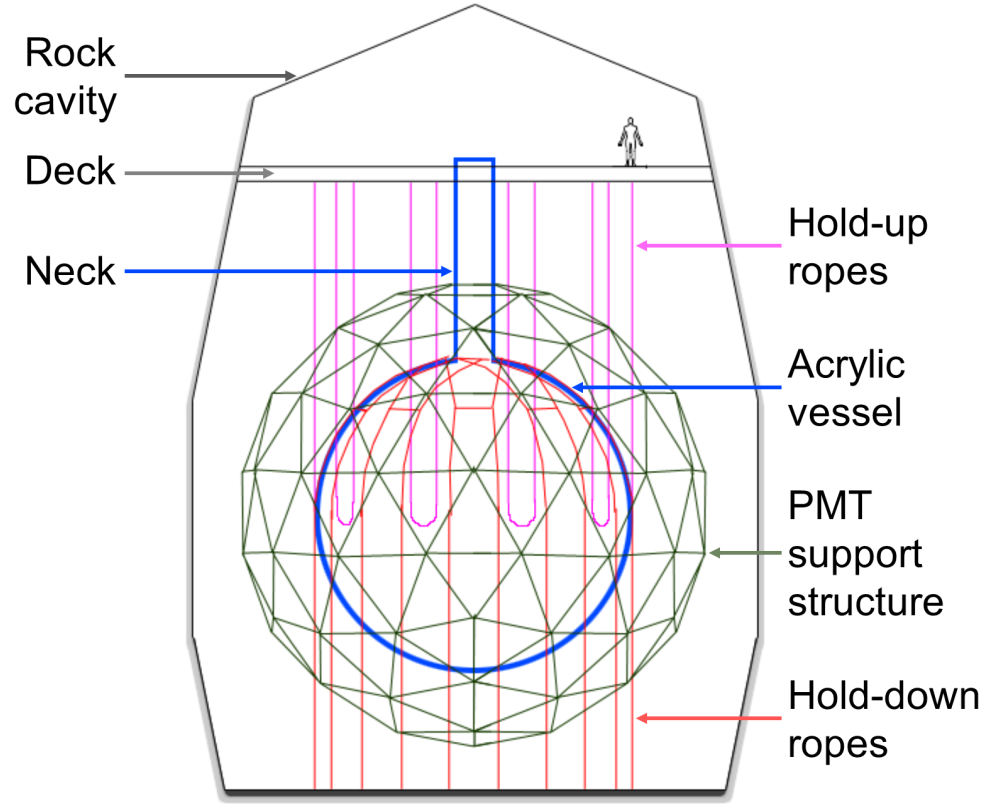
\includegraphics[width=10cm]{SNOPdetector.png}
	\caption[The SNO+ detector labeled with main structures.]{The SNO+ detector labeled with main structures, modified from Ref.~\cite{jones2011background}.}
	\label{snopdetector}
\end{figure}

\section{SNO+ Physics Phases}\label{sect:physicsPhase}
The SNO+ experiment is designed for multi-purpose measurements of neutrino physics. The detector has been running since December 2016. There are three physics phases of the experiment and each phase has different detection media inside the AV: the water phase, the scintillator phase, and the tellurium phase\cite{whitepaper}. 

\subsection{Water Phase} \label{sect:waterPhase}
In this initial phase, about 905 tonnes of ultrapure water was filled into the AV. The detector collected water physics data from May 2017 to July 2019.

During the data-taking, different types of calibration runs have been taken. The detector timing and energy response, systematics, and backgrounds are studied. Multiple physics analyses of invisible nucleon decay, solar neutrinos, and reactor antineutrinos are ongoing, and relating results have been published\cite{anderson2019search,anderson2019measurement,anderson2020measurement,anderson2021optical}. The external backgrounds are also measured, which will be the same as the following two phases.

In this phase, the main physics goal is to search for the invisible nucleon decay, which violates the baryon number and predicts Grand Unified Theory (GUT).  A proton or a bound neutron decays away without releasing charged particles in the invisible decay mode, compared to the ``visible'' decay channels of $p\to e\pi$ and $p\to\nu K$, which has been searched and set limits by the SuperK experiment. In the SNO+ water detector, $^{16}$O may decay into $^{15}$O$^*$ (bound neutron invisible decay) or $ ^{15}$N$^*$ (proton invisible decay) excited state. The $^{15}$O$^*$ has 44\% chance to deexcite to produce 6.18 MeV $\gamma$ ray and 2\% chance to produce 7.03 MeV $\gamma$; while $^{15}$N$^*$ has 41\% to release 6.32 MeV $\gamma$ and 7.01, 7.03 and 9.93 MeV $\gamma$ with chances of 2\%, 2\% and 3\% respectively. The experiment has searched for these $\gamma$ signals and the first publication sets world-leading limits of $\mathcal{O}(10^{29})$ years for both the proton and neutron invisible decay lifetime at 90\% Bayesian credibility level\cite{anderson2019search}. 

The $^8$B solar neutrinos were measured with a 69.2 kilo-tonnes$\cdot$day dataset. By analyzing the solar neutrino elastic scattering events based on the dataset (Chapter 6 will discuss the method in detail), the number of the solar neutrino events were counted in different energy regions. In the first publication\cite{anderson2019measurement}, by fitting to the non-oscillation solar neutrino model, an observed flux was obtained from the dataset to be $2.53^{+0.31}_{-0.28}(stat.)^{+0.13}_{-0.10}(syst.)\times 10^6$ cm$^{-2}$s$^{-1}$ for the $^8$B solar neutrinos with energies larger than 5 MeV. In the energy region larger than 6 MeV, the dataset has a background rate of $0.25^{+0.09}_{-0.07}$ events/kilo-tonne$\cdot$day, which is extremely pure with solar neutrinos. Currently, this background rate is the lowest one compared to the other water Cherenkov detectors\cite{anderson2019measurement}. 

Reactor antineutrinos can be captured by the SNO+ detector and get measured. 40\% of these antineutrinos are from one nearby reactor complex in Canada at a 240-km baseline; 20\% are from two Canadian complexes at around 350 km; the rest are from the USA and elsewhere with longer baselines\cite{whitepaper}. Though the antineutrino event rate in pure water is much lower than in the scintillator, during the water phase, SNO+ still has the potentials to detect reactor antineutrinos due to the low background dataset and relatively high detection efficiency. An Americium-Beryllium (AmBe) calibration source was deployed during the water phase to evaluate the sensitivity for detecting reactor antineutrinos.  This source provides neutrons along with 4.4-MeV $\gamma$s. Neutrons are captured by hydrogen, and 2.2-MeV $\gamma$s are released. An analysis of delayed coincidence between 4.4-MeV and 2.2-MeV $\gamma$s can help tag neutrons, which is crucial for tagging the reactor antineutrinos since they are measured by the inverse $\beta$-decay process, which produces neutrons with a similar energy scale. In the first publication for the SNO+ water phase, a neutron detection efficiency of 50\% was obtained when the AmBe source was deployed at the center of the detector; the neutron-hydrogen capture time constant $\tau$ was measured to be $202.35_{-0.76}^{+0.87}~\mu s$, and from $\tau$, a thermal capture cross-section was calculated to be $336.3^{+1.2}_{-1.5}$ milli-barn (mb)\cite{anderson2020measurement}.


%During the period from October 2018 to July 2019, over 20 tonnes of LAB (without PPO) was filled into the detector and the liquid mostly occupied the neck volume, slightly below the neck bottom. With the nitrogen cover gas on the top, the data taken during this period is considered as low background data.
\subsection{Partial-fill Phase} \label{sect:partialPhase}
%This partially filled transition phase (called the ``partial-fill'' phase) is mainly aimed to understand the in-situ backgrounds of the scintillator. 
%A six to twelve months of data-taking are expected for this phase. 
%During the filling, the partially-filled detector has been operated at several different water level (mainly at 5.7 m, 0.75 m)

\subsection{Scintillator Phase} \label{sect:scintPhase}

In this phase, the AV will be filled with 780 tonnes of liquid scintillator, which is a mixture of linear alkylbenzene (LAB) as a solvent and 2 g/L of 2,5-diphenyloxazole (PPO) as a fluor. This LAB-based organic liquid scintillator is referred to as the ``unloaded'' liquid scintillator (Sect.~\ref{sect:LS_SNO+} will discuss more details).

The main physics goal of the scintillator phase is to measure low energy solar neutrinos: the CNO, pep, and low energy $^8$B neutrinos. The pep neutrinos are mono-energetic, with $E_\nu$=1.442 MeV and their flux is well predicted by the Standard Solar Model\cite{davini2016cno}. A measurement of the pep neutrinos will give more information on the matter effects in neutrino oscillations. 

The solar metallicity is the abundance of elements heavier than $^4$He (called ``metal'' elements in the context of astronomy). It is poorly constrained and the predictions from different solar models disagree with each other. A measurement of the CNO neutrinos can give the abundance of $^{12}$C, $^{13}$N and $^{15}$O and can thus resolve the metallicity problem\cite{cerdeno2018cno}.

Three kinds of antineutrinos will also be measured: reactor antineutrinos as mentioned before; geoneutrinos from natural radioactivity in the Earth; and the supernova neutrinos. SNO+ is planned to join the SuperNova Early Warning System (SNEWS), which is an international network of experiments with abilities to provide an early warning of a galactic supernova\cite{snop_jinst}.

\subsubsection{Tellurium Phase} \label{sect:tePhase}
In this final phase, 0.5\% natural Tellurium (Te) by mass (with 1.3 kilo-tonnes of $^{130}$Te) will be loaded into the scintillator, which is referred to as the ``Te-loaded'' scintillator (Sect.~\ref{sect:TeLS_SNO+} will discuss more details). Higher loading concentrations would be possible for a further loading plan\cite{Paton:2019kgy}. The main purpose of this phase is to search for the $0\nu\beta\beta$ signals in $^{130}$Te.

\section{Detection Media} \label{sect:detectionMedia}
In the SNO+ detector, charged particles are expected to interact with the detection media and create Cherenkov lights and scintillation lights. 

\subsection{Cherenkov Radiation}
For any charged particle traveling in a transparent medium at an ultra-relativistic speed (a speed greater than the local phase speed of light in the medium),  a kind of electromagnetic radiation, called Cherenkov radiation, can be emitted from the coherent response of the medium under the action of the field of the moving particle\cite{jackson2007classical,landau2013electrodynamics}.

Suppose a charged particle moves in a transparent, isotropic, and non-magnetic medium and creates an electromagnetic wave. The electromagnetic wave propagates with a wavenumber $k=n\cdot\omega/c$, where $c$ is the speed of light in vacuum, $n$ is the real-valued refractive index and $\omega$ is the frequency. If the particle travels uniformly along x-axis with a velocity of $v$, the x-component of the wave vector is $k_x=\omega/v$. For a freely propagating wave, $k>k_x$, therefore $v>v_p=c/n(\omega)$, where $v_p$ is the phase velocity in the medium. Under this condition that the speed of the charged particle is greater than the $v_p$, the Cherenkov radiation is emitted with a frequency of $\omega$\cite{landau2013electrodynamics}.   

The Cherenkov angle, $\theta_c$ is the angle between the direction of the particle and the direction of Cherenkov emission and it is well-defined by $\cos\theta_c(\omega) = \frac{c}{n(\omega)v}$. The radiation is distributed over a surface of a cone with the half-opening angle $\theta_c$. 

Consider the condition $v>v_p=c/n(\omega)$, for the case of $e^-$ traveling in a water detector, if neglecting the dependency on $\omega$, $n_{water}\simeq 1.33$ \cite{pdg2020}, then $\theta_c\simeq 41.25^\circ$ and $v_p\simeq 2.254\times10^8~m/s$, which corresponds to a kinetic energy $E_k=(\gamma-1)mc^2=0.264~MeV$ for $e^-$, where $\gamma=1/\sqrt{1-v_p^2/c^2}$. This is the lowest kinetic energy to create Cherenkov radiation, which is referred to the Cherenkov threshold ($E_{thresh}$). In the case that the LAB-PPO liquid scintillator is the medium, $n\simeq 1.50$\cite{tseung2011ellipsometric}, $\theta_c\simeq 48.19^\circ$ and for $e^-$, $E_{thresh}\simeq 0.175~MeV$.   

For a particle with a charge of $ze$, the number of photons produced by Cherenkov radiation per unit path length and per unit frequency of the photons is given by\cite{leo2012techniques}:
\[
\frac{d^2N}{d\omega dx}=\frac{\alpha^2 (ze)^2}{c}\sin^2\theta_c=\frac{z^2\alpha}{c}(1-\frac{1}{\beta^2 n^2(\omega)}),
\]
where $\alpha$ is the fine structure constant.

Transforming the frequency into the wavelength ($\lambda=2\pi\omega$) and integrating over the wavelength, the number of photons along the particle track projected on the x-axis is\cite{leo2012techniques}:
\[
\frac{dN}{dx}=2\pi (ze)^2\alpha\sin\theta_c\int_{\lambda_1}^{\lambda_2}\frac{d\lambda}{\lambda^2},
\]

For optical photons with wavelengths ranging from $350$ to $550~nm$ (typical PMT detection sensitive range), the above formula can be calculate into\cite{leo2012techniques}:
\[
\frac{dN}{dx}=476(ze)^2\sin^2\theta_c~photons/cm.
\]

For the Cherenkov radiation caused by $e^-$ in a water detector, $dN/dx \simeq 207~photons/cm$; while in the LAB-PPO case, $dN/dx \simeq 264~photons/cm$. In a realistic measurement, the detection efficiency and the coverage of photon sensors are also required to be taken into account.

\subsection{Scintillation from Organic Scintillator}

Besides the Cherenkov photons described in the previous section, the majority of lights emitted from the organic scintillator are scintillation photons.

The organic liquid scintillator can convert the kinetic energy of charged particles into scintillation photons with wavelengths in the sensitive detection region of PMTs. They are aromatic hydrocarbon compounds with benzene-ring structures. When ionizing radiation happens in the scintillator, the free valence electrons of the molecules are excited and transit to occupy the $\pi$-molecular orbitals with the benzene rings. These highly delocalized electrons are called $\pi$-electrons, which can occupy a series of energy levels. A Jablonski diagram, invented by Polish physicist Aleksander Jab\l o\'{n}ski, is generally used to describe molecular absorbance and emission of light. In Fig.~\ref{jablonski}, the Jablonski diagram illustrates the $\pi$-electronic energy levels of an organic scintillator molecule\cite{knoll2010radiation,leo2012techniques}. 
\begin{figure}[!htb]
	\centering
	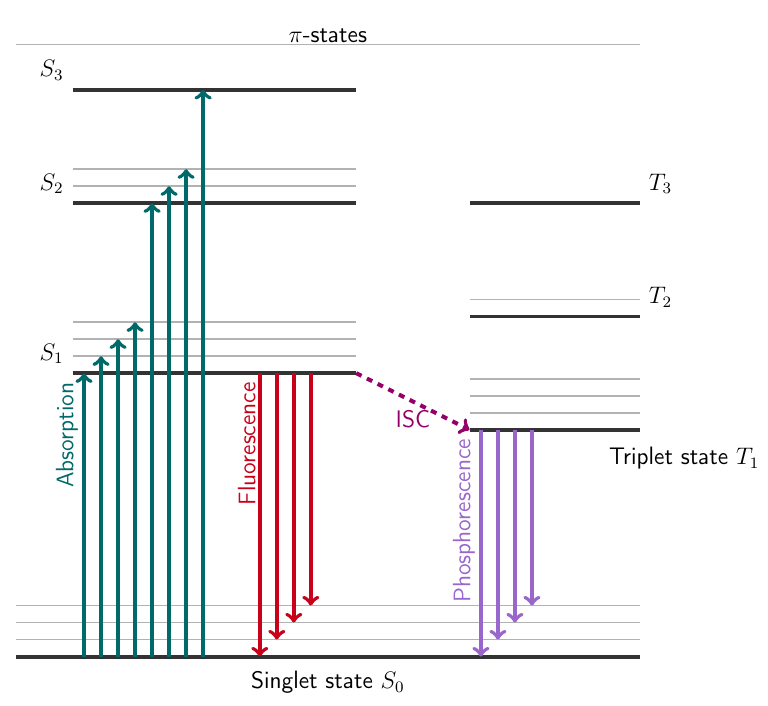
\includegraphics[width=10cm]{jablonski.png}
	\caption[A Jablonski diagram for the organic scintillator.]{A Jablonski diagram for the organic scintillator, modified from Refs.~\cite{birks1965theory, knoll2010radiation}.}
	\label{jablonski}
\end{figure}

In the diagram, $S_{0,1,2,3,...}$ are the energy levels of the spin-0 singlet states, where $S_0$ is the ground state and $S^*=S_{1,2,3,...}$ are the excited singlet states. Above the ground state $S_0$, there is also a set of spin-1 triplet states $T_{1,2,3,...}$, where $T_1$ is the lowest triplet state. These electron energy levels are labeled with thick black lines. The energy spacings between these levels are $\mathcal{O}(eV)$. In each level, there are also fine structure levels that correspond to excited vibration modes of the molecule (labeled with gray lines and can be marked as $S_{10}, S_{11}, ..., S_{20}, S_{21}, ...$). The energy spacing between these fine levels are $\mathcal{O}(0.15~eV)$\cite{leo2012techniques, knoll2010radiation}.

The ionization radiation transfers the energy to the molecules and excites the electron levels as well as the vibrational levels, labeled as the absorption lines (in green). The decays between the excited singlet states (not to the ground state) are almost immediate ($\leq 10~ps$) without the emission of light. This process is called internal degradation. The decays from the excited singlet state $S_1$ (as well as the vibrational states $S_{10},S_{11},S_{12},...$) to the ground state (as well as the vibration states $S_{01}, S_{02}, ...$) happen promptly ($\mathcal{O}(ns)$) and emit lights (labelled as red lines). This process is called fluorescence which contributes to the prompt component of the emission of scintillation light. The probability of $S_1$ decays into the vibrational states $S_1 \to S_{01},S_{02},...$ among the ground state is more than $S_1\to S_0$. Since the absorbed energy of $S_0 \to S_1$ is larger than the emitted energy of $S_1 \to S_{01}, S_{02},...$, the scintillators have very little self-absorption of the fluorescence and are transparent to their own radiation. The effect of Stokes shift, which refers to the overlap between the optical absorption and emission spectra, is small for the organic scintillator\cite{leo2012techniques,knoll2010radiation}. 

The transitions between the singlet and triplet states are highly forbidden due to the
electron spin-flip is involved\cite{von2015measurement,sorensen2016temperature}. There also exists a relatively rare process called intersystem crossing (ISC), which converts excited singlet states into triplet states. Besides this, 75\% of triplet states can be produced by ionization-recombination\cite{von2015measurement,dunger2018topological}.

For the de-excitation, the similar processes of internal degradation occur among $T_{2,3, ...} \to T_1$. $T_1$ is a relatively stable state and the lifetime of the molecule in the triplet state is in $\mathcal{O}(10^{-4}~-~10~s)$\cite{mcquarrie1997physical}. $T_1\to S_0$ is highly forbidden. However, the $T_1$ state can go through an indirect decay process by interacting with another excited $T_1$ molecule and forms an excited singlet state:
\[
T_1+T_1\to S^*+S_0+phonons
\]
The $S^*$ will de-excite and emit delayed scintillation light. The process for emitting this delayed scintillation light is called delayed fluorescence or phosphorescence\cite{leo2012techniques}. This process contributes to the delayed component of scintillation light.

For a typical scintillator detector, the time scale of detector response is $\mathcal{O}(1-100~ns)$. In this time region, the emission of the scintillation light contains the primary fluorescence from the de-excitation of the singlet states (prompt component) and the delayed fluorescence from the de-excitation of the indirect triplet states (delayed component)\cite{dunger2018topological}. The time profile of the scintillation light emission is a mixture of prompt and delayed components. 

Different charged particles can cause different ionization densities when they deposit energies to the scintillator molecules. The ionization density affects the relative population of the excited singlet and triplet states. Compared to an $e^-$, an $\alpha$ particle can cause a high ionization density, which produces a higher ratio of triplet states. Therefore, the time profile for the $\alpha$ particle has more delayed components or longer tails than the $e^-$. This enables the organic scintillator to distinguish $\alpha$ with $e^-$ or other lighter charged particles\cite{dunger2018topological, collaboration2020development}. 

An empirical formula, called follows Birk's law\cite{birks1951scintillations, birks1965theory}, describes the photon yield along with unit distance by the incident particle:
\[
\frac{dY}{dx}=A\frac{dE/dx}{1+k_B\cdot dE/dx},
\]
where $A$ is a normalization constant, $k_B$ is the Birks' constant of the scintillator, which in practice is obtained by fitting the formula to the measured data.

\subsection{Liquid Scintillator for SNO+}\label{sect:LSproperty}
Organic scintillators can release a large number of photons with wavelengths in the sensitive regions of the PMTs and have abilities for particle identification. In addition, since organic liquids are non-polar media, it is hard for ionic impurities to dissolve in. This leads to the lower contamination levels of uranium (U), thorium (Th), and potassium (K) in the organic liquid scintillators. Among the organic scintillators, aromatic organic liquid scintillators have high electron densities and thus they can provide sufficient targets for particle interactions\cite{PerkinElmer}. Due to these advantages, aromatic organic liquid scintillators have been extensively developed as detection media for large particle detectors, especially for neutrino experiments, such as KamLAND, Borexino, Day Bay, and JUNO\cite{collaboration2020development}.

SNO+ has developed such kind of liquid scintillators that are compatible with the detector components, especially with the acrylic materials, like the AV sphere. Two kinds of SNO+ liquid scintillators are discussed in the following sub-sections: the unloaded liquid scintillator for the scintillator phase and the Tellurium-loaded liquid scintillator (TeLS) for the tellurium phase.

\subsection{Water-based Wavelength Shifter (Proposal)}\label{sect:wbWLS}
X. Dai et al.\cite{dai2008wavelength} made a proposal for adding wavelength shifters (WLS) into a water Cherenkov detector like SNO. Compared to the water Cherenkov detector, a water-based wavelength shifter (wbWLS) detector has a higher light yield (about threefold higher than SNO\cite{dai2008wavelength}) and thus lowers down the energy threshold and opens opportunity to detect low energy events. At the meantime, it will still keep the directionality from Cherenkov signals compared to a loss of the directionality for the liquid scintillator detector, which can be used to suppress the backgrounds when analyzing directional signals, such as solar neutrinos. This technology is being studied by future neutrino experiments, such as the Advanced Scintillation Detector Concept (ASDC)\cite{alonso2014advanced}, WATCHMAN experiment\cite{askins2015physics} and Jinping experiment\cite{beacom2017physics}.

There was a proposal of adding wavelength shifter (WLS) into the SNO+ detector in the middle of the water phase, made by the University of Alberta group. The specific wavelength shifter we considered is PPO, which is a well-studied ingredient of the liquid scintillator used in the SNO+ scintillator phase and Te-loaded phase. Although this proposal was not adopted due to the experiment schedule, it is still worthwhile for a conceptual study of a SNO+-like detector that uses water-based wavelength shifter (wbWLS) as detection medium.

In Chapter 4, a vertex reconstruction method is discussed. 

\subsubsection{Unloaded Liquid Scintillator}\label{sect:LS_SNO+}
SNO+ adopts a scintillator cocktail contains two primary components: LAB as solvent and PPO as solute. LAB is doped with PPO to a concentration of 2 g/L. Fig.~\ref{labppo-molecule} shows the chemical structural formulae of LAB and PPO\cite{collaboration2020development}.
\begin{figure}[!htb]
	\centering
	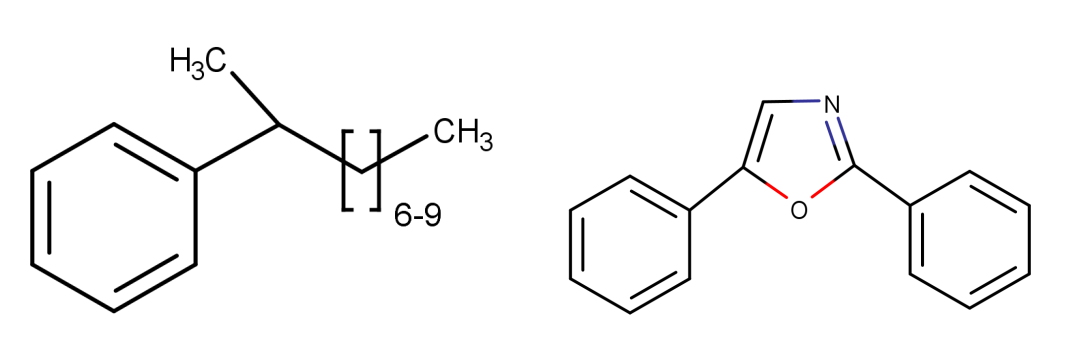
\includegraphics[width=8cm]{lab-ppo-molecule.png}
	\caption[Structural formulae of LAB and PPO.]{Structural formulae of LAB (left) and PPO (right).}
	\label{labppo-molecule}
\end{figure}

LAB is a family of alkylated aromatic organic compounds with a phenyl group attached to a long carbon chain varying from 9 to 14 carbons\cite{wiki_LAB, collaboration2020development}. It has been used as a biodegradable detergent since the 1960s and it is proved to be relatively non-toxic and very low risks for the environment or human health\cite{wiki_LAB}. Due to the long carbon chain, LAB is an effective energy absorber.
close to linear response to energy


Good stability and chemically compatible




High light yield and attenuation length.


attenuation length
good optical transparency 

 flash point at 140 $^\circ C$

 It has very low levels of natural radioactive contaminants such as U, Th and K.
The target background levels for the SNO+ LAB are expected to be $\mathcal O(10^{-17})$ gram of $^{238}$U in per gram LAB (g$^{238}$U/gLAB), which is equal to be thousands of events per year;
The $^{232}$Th and $^{40}$K levels are $\mathcal O(10^{-17})$ g/gLAB, which is equal to be hundreds of events per year\cite{markchen_bkg}.


It has fast timing response different timing spectrum for $\alpha$ and $\beta$ events, which enables an $\alpha/\beta$ discrimination. 
High flash point and low toxicity for lab safety.
 appropriate density for mechanical stability
 Low cost.


The LAB used by SNO+ is provided by CEPSA Qu\'{i}mica B\'ecancour Inc.



%Kosswig, Kurt (2005). "Surfactants". Ullmann's Encyclopedia of Industrial Chemistry. Wiley-VCH. doi:10.1002/14356007.a25_747. ISBN 3527306730.


As a wavelength shifter, PPO is usually added and dissolved into the LAB \cite{wunderly1990new}. This wavelength shifter is used as a fluor. Energies are transferred from LAB to PPO via non-radiative F{\"o}rster resonant energy transfer. It can shift the wavelengths of the scintillation photons to a range of 300-550 nm, which is in the sensitive range of the PMT detection and can also reduce the probability of being the self-absorption of LAB.

A 2 g/L PPO concentration in LAB is optimized by SNO+\cite{whitepaper}. The absolute light yield of the LAB-PPO liquid scintillator has been well-measured from large particle physics experiments \cite{xing2015preliminary}, borexino], as well as bench-top measurements \cite{xing2015preliminary,kaptanoglu2019cherenkov, novikov}. The absolute light yield of the LAB+2g/L PPO liquid scintillator determined by SNO+ is 11900 photons/MeV\cite{grullon2014light}. And this light yield is expected to be increased by over 15\% after extensive purification process\cite{snop_jinst}. 


Fig.~\ref{absLength} shows absorption lengths.

\begin{figure}[!htb]
	\centering
	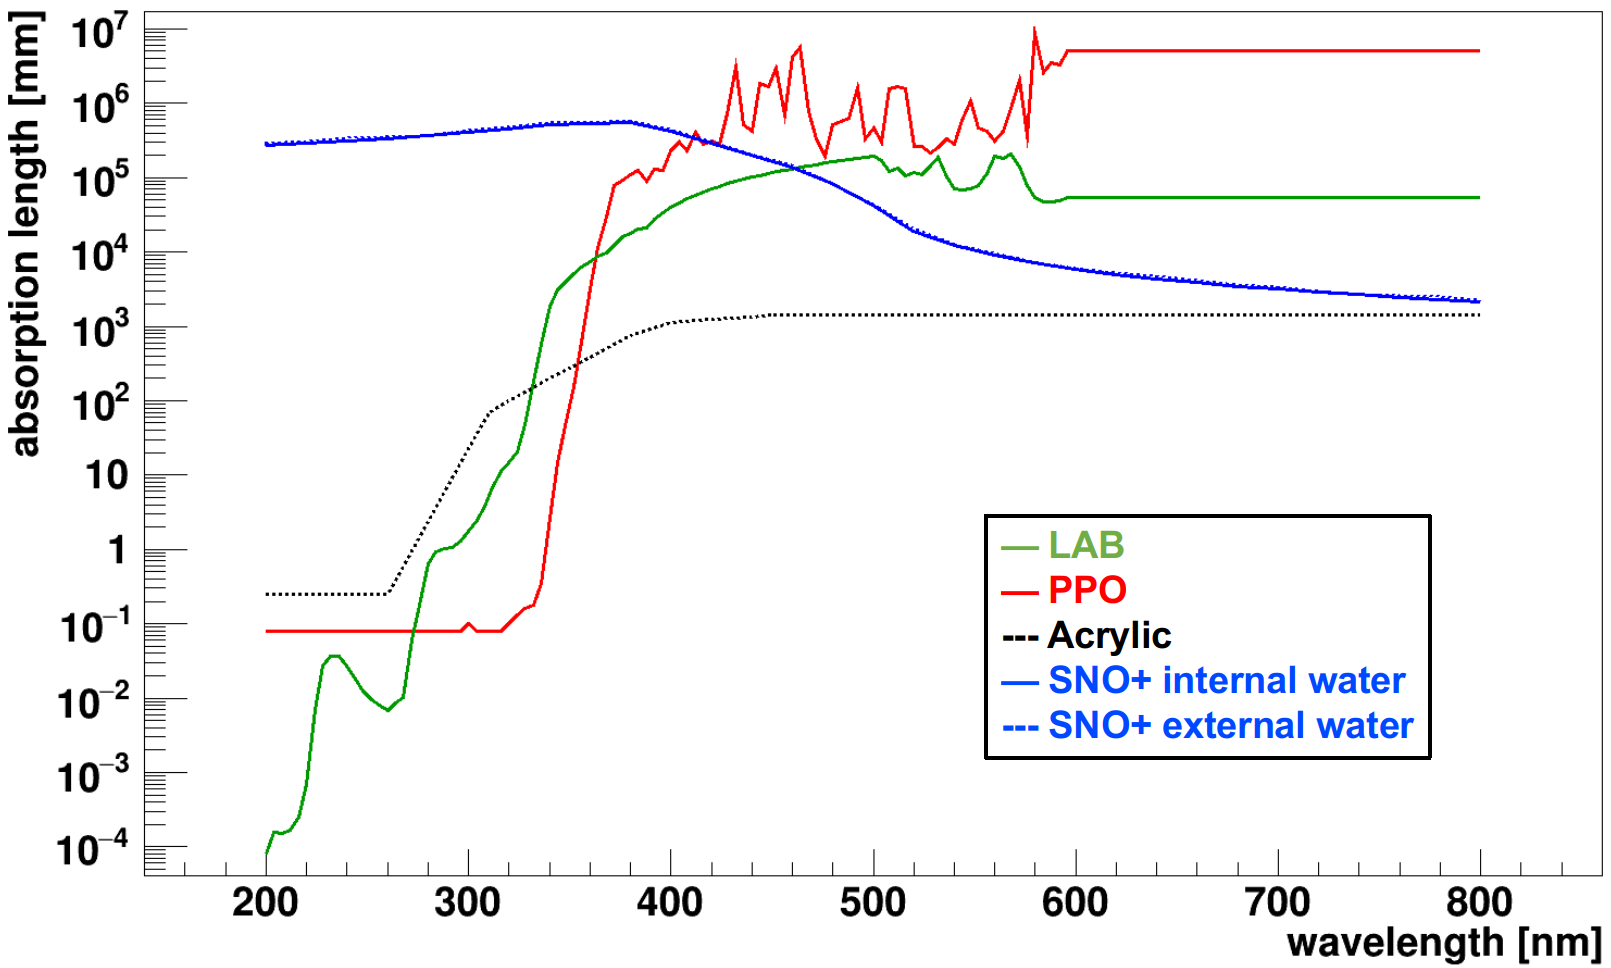
\includegraphics[width=10cm]{absLength.png}
	\caption[Absorption length of SNO+ optical components.]{Absorption length of SNO+ optical components. The internal (solid blue line) and external water (dashed blue line) absorption curves are based on the measurements of the laserball scans in July 2018 during the SNO+ water phase. The horizontal lines are due to absence of the measurements and they are conservative assumptions.}
	\label{absLength}
\end{figure}

%non-radiative transfer from LAB (solvent) to PPO (fluor)
%the non-radiative transfer efficiency for 2g/L PPO in LAB is measured as $78.2\pm 1.5~\%$
%the transfer efficiencies

This transfer efficiency ($\mathcal{\epsilon}_{transfer}$) increases as the PPO concentration increasing, as shown in the Table. Above the 2 g/L concentration, the light yield reaches a plateau
\cite{collaboration2020development}.


The optical response of the liquid scintillator.

The time profiles of scintillator were obtained from bench-top measurement. 
An empirical model consists $n$ ($n=3~or~4$) exponential decays  with a common rise time is used to describe the time profiles\cite{biller2020slow}.

Default timing fitting functions:
\[\sum^{n}_{i=1}A_i\cdot\frac{e^{-\frac{t}{\tau_i}}-e^{-\frac{t}{\tau_{rise}}}}{\tau_i-\tau_{rise}}
\]

while the rise time, $t_{rise} = 0.8~ns$ the timing parameters $t_i$,
amplitude $a_i$ are determined by the bench-top measurements \cite{chicagoTiming}.




\begin{table}[ht]
	\centering
	\begin{tabular}{cc}
		\toprule
		PPO concentration (g/L) & $\mathcal{\epsilon}_{transfer}$(\%)	\\
		\midrule
		4   & $86.0\pm 0.8$\\
		2  & $78.2\pm 1.5$\\
		1  & $67.7\pm 2.3$\\
		0.5 & $59.3\pm 3.2$\\
		0.25 & $48.7\pm 5.0$\\
		\bottomrule
	\end{tabular}
	\label{transfer_efficiency}
\end{table}

%T. Kaptanoglu. Measurements of light yield and timing of 0.5 g/L LAB+PPO. SNO+ Internal Document (docDB-5997-v1).
%T. Kaptanoglu. Timing and light yield measurement of Te+DDA LAB+PPO. SNO+ Internal Document (docDB-4813-v4).
%T. Kaptanoglu. Penn Light Yield Measurements of Te+DDA samples. SNO+ Internal Document (docDB-5124-v2).

\begin{table}[ht]
	\caption[]{scintillator $\alpha/\beta$ timing parameters\cite{tanner0p5,joshW1,chicagoTiming}.}	\label{scint_timing} 
	\centering
	\begin{tabular*}{165mm}{c@{\extracolsep{\fill}}*9c}
		\toprule 
		\multicolumn{1}{c}{scintillator} & \multicolumn{4}{c}{timing [ns]} & \multicolumn{4}{c}{amplitudes}\\
		\cline{0-1}\cline{2-5} \cline{6-9}		
		particles      & $t_1$ & $t_2$ & $t_3$ & $t_4$ & $a_1$ &$a_2$ &$a_3$&$a_4$\\
		\midrule
		\multicolumn{9}{l}{LAB + 2g/L PPO (default scintillator)}\\
		$e^-$ & 4.88 & 15.4 & 66.0 & 400 & 0.665 & 0.218 & 0.083& 0.0346\\	
		$\alpha$ & 4.79 & 18.4 & 92.0 & 900 & 0.427 & 0.313 & 0.157 & 0.1027\\
		\hline
		\multicolumn{9}{l}{LAB + 0.5g/L PPO (partial-fill phase)} \\
		$e^-$& 7.19 & 24.81 & 269.87 & -- &0.553 &0.331 &0.116 & --\\
		$\alpha$& 6.56 &23.82 &224.19&--& 0.574&0.311& 0.115&--\\
		\hline
		\multicolumn{9}{l}{LAB + 2g/L PPO + 0.5\% molar concentrations DDA} \\
		$e^-$ & 5.0& 12.1& 33.3& 499.0& 0.68& 0.21& 0.07& 0.04\\
		$\alpha$ &3.8 &11.3& 65.3& 758.0& 0.48& 0.32& 0.14& 0.06 \\
		\hline
		\multicolumn{9}{l}{LAB + 2g/L PPO + 0.5\% molar concentrations Te+0.5\% molar DDA}\\
		$e^-$ & 3.7 & 10.0 & 52.0  & 500.0 & 0.72 & 0.23 & 0.02 &0.03\\
		$\alpha$ & 3.69 & 15.5 & 79.3  & 489.0 & 0.63 & 0.23 & 0.07 &0.07\\	
		\bottomrule	
	\end{tabular*}
\end{table}

\begin{figure}[!htb]
	\centering
	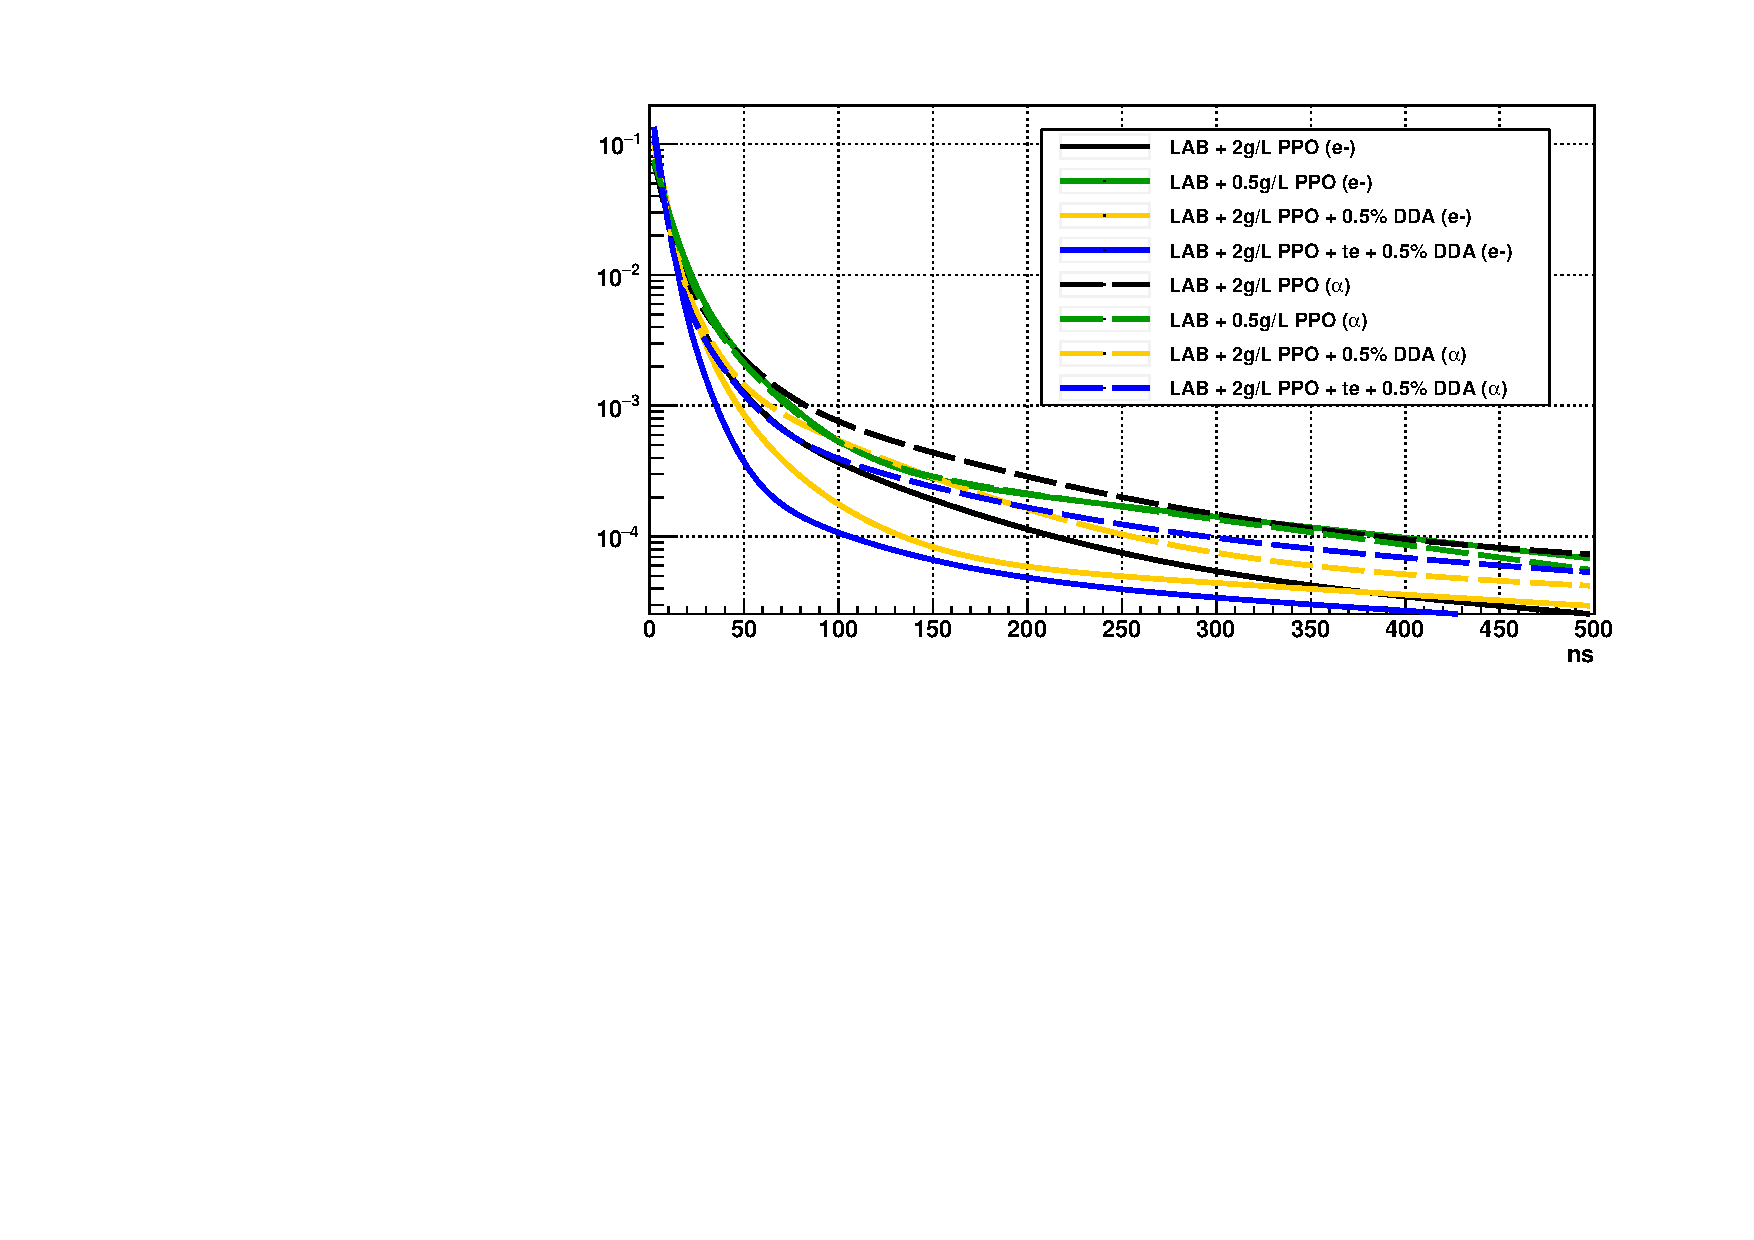
\includegraphics[width=10cm]{plotAllTiming.pdf}
	\caption{Timing profiles for liquid scintillators in different SNO+ phases.}
	\label{allTiming}
\end{figure}

\subsubsection{Tellurium-loaded Liquid Scintillator}\label{sect:TeLS_SNO+}

To load the $^{130}$Te into the liquid scintillator, an organo-metallic compound, called the ``Tellurium Butanediol (TeBD)'', is formed by 
condensation (or called ``diolization'') reactions between telluric acid (TeA) and 1,2-butanediol (BD)\cite{Paton:2019kgy}. A tertiary amine: N, N-Dimethyldodecylamine (DDA) was added during the reaction to stabilize TeBD compounds and avoid any phase separation\cite{teLoadingPaper}. Fig.~\ref{fig:paton_te} shows initial stages of the process. This compound is then loaded into the liquid scintillator.
\begin{figure}[!htb]
	\centering
	
\includegraphics[height = 3cm]{TeBD_process.png}
	\caption{Initial stages of the TeBD compound formation, modified from Ref.~\cite{Paton:2019kgy}.}
	\label{fig:paton_te}
\end{figure}

Two synthesis procedures, the DDA and SOP procedures, are being developed by the SNO+ Tellurium-loading working groups\cite{biller2017new,teDDA,DDAvsSOP}.

These method allow the optical transparency of the scintillator to be conserved. 
The total light yield of the full cocktail is expected to be 400 NHits/MeV 

Tellurium-loaded 65\% of the pure, unloaded scintillator

water-based wavelength shifter

timing profile, the intensity of scintillation light as a function of time

the prompt fluorescence intensity at a time $t$ excitation be $I=I_0e^{-\frac{t}{\tau}}$

singlet and triplet states 
ionization density 
depend
$\alpha$-particle
high ionization density 
quenching, 


2 g/L PPO gives an absolute light yield of 11900 photons/MeV.


for the partial-fill phase, 0.5 g/L PPO gives Measurements in 0.5 g/L showed a light yield of 52\% of 2 g/L,  
6190 photons/MeV\cite{tanner0p5,joshW1}.

For the $^{130}${Te} $0\nu\beta\beta$-decay process, the signature energy peak is at $2.5~MeV$\cite{whitepaper}. This peak is relatively small and can be immersed in the ubiquitous radioactive decays from natural sources, such as the natural Uranium and thorium decay chains existing in the materials\cite{whitepaper}. Therefore, the $0\nu\beta\beta$-decay experiments require a very high energy resolution to distinguish the signal from the backgrounds. For the liquid scintillator, it is expected to create as large amount of light caused by a particle interaction as possible. A quantity of light yield, defined as the number of photons for per MeV energy deposit (photons/MeV) by a particle interaction, is used for describing the detection property of the liquid scintillator.

To meet the low background requirement of the $0\nu\beta\beta$ analysis, the purity of the TeLS cocktail is aimed to $\mathcal{O}(10^{-15})$ g/g level for U and Th. 

\subsection{Relative Light Yield Measurements of the Te-loaded Liquid Scintillators}
As mentioned in the previous section, the $0\nu\beta\beta$ analysis requires high purity and a good light yield of the TeLS. %%% add more

Here we measured the light yield of $0.5\%$ Te-loaded LAB (TeLS) samples relative to the LAB-PPO scintillator (relative light yield, RLT). With tellurium loading into the LAB, the light yield of the liquid scintillator will go down since the tellurium atoms can block the photon transmissions to the photosensors.  The light yield of the TeLS is crucial for the $0\nu\beta\beta$-decay experiments since it determines the energy resolution. It is also crucial for the experiments that are aimed to develop high light yield Tellurium-loaded scintillators\cite{biller2017new}.

\subsubsection{Measurement Setup and Data Acquisition}

We first prepared LAB+2 g/L PPO by dissolving PPO into the pure LAB. The LAB-PPO mixture was distilled by heating and flowing with liquid nitrogen to remove humidity and oxygen, affecting the light yield for 48 hours. The distilled LAB-PPO was added into the original 16.5\% weight Te-butanediol samples to dilute into the 0.5\% TeLS samples. Te-butanediol samples from both of the DDA and SOP synthesis procedures were prepared. They are referred to as TeDDA and TeSOP samples, respectively. These samples were further transferred into scintillation vials for the measurement. These vials have PTFE caps sealed on the top of the glass cylinders. The liquid level for each sample was kept at 30 mm to avoid air bubbles created by squeezing the vial cap into the liquid. The dimensions of the vial are shown in the left picture of Fig.~\ref{scintVial}.

\begin{figure}[htbp]
	\subfigure{
		\begin{minipage}[t]{0.38\textwidth}
			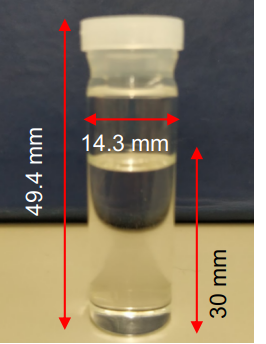
\includegraphics[width=4cm]{scintVial.png}
		\end{minipage}
	}   
	\subfigure{
		\begin{minipage}[b]{0.35\textwidth}
			\centering
			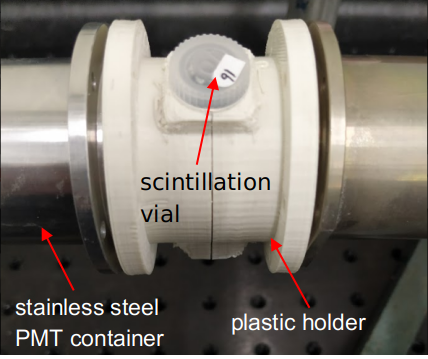
\includegraphics[width=6cm]{plasticHolder.png}
		\end{minipage}
	}
	\caption[A vial of the test sample and the measurement setup.]{A vial of the test sample (left) and the measurement setup (right). Left: The samples were filled into scintillation vials. The dimensions are shown in the picture. Right: two PMTs were aligned to face to the scintillation vial from each side.}
	\label{scintVial}
\end{figure}

Two Hamamatsu R580 PMTs \cite{pmtR580} were used for detecting the light. The diameter of the PMT round surface is 38.71 mm. These PMTs were housed in stainless steel cylinders (PMT holders), set face to face, looking at the scintillation vial from each side. The PMTs and the vial were aligned by a plastic piece, as shown in the right picture in Fig.~12.  The plastic piece is cylindrical with a hole on the top to plug in the scintillation vial and a slot at the bottom to attach a radioactive source. Inside the cylinder, there is a button-shaped groove at the bottom to fix the vial plugged in and keep the vial upright. Also, a 2-mm-diameter hole was drilled at the bottom of the piece to allow the radiation rays to pass through the vial from the bottom. The surface inside was polished to reduce the absorption of the material to the photons. The piece is made of plant-based and biodegradable polylactide (PLA) filament and was machined by a 3D printing facility at the University of Alberta. The pictures of the pieces are shown in Fig.~\ref{scintVial}.

\begin{figure}[htbp]
	\centering	
	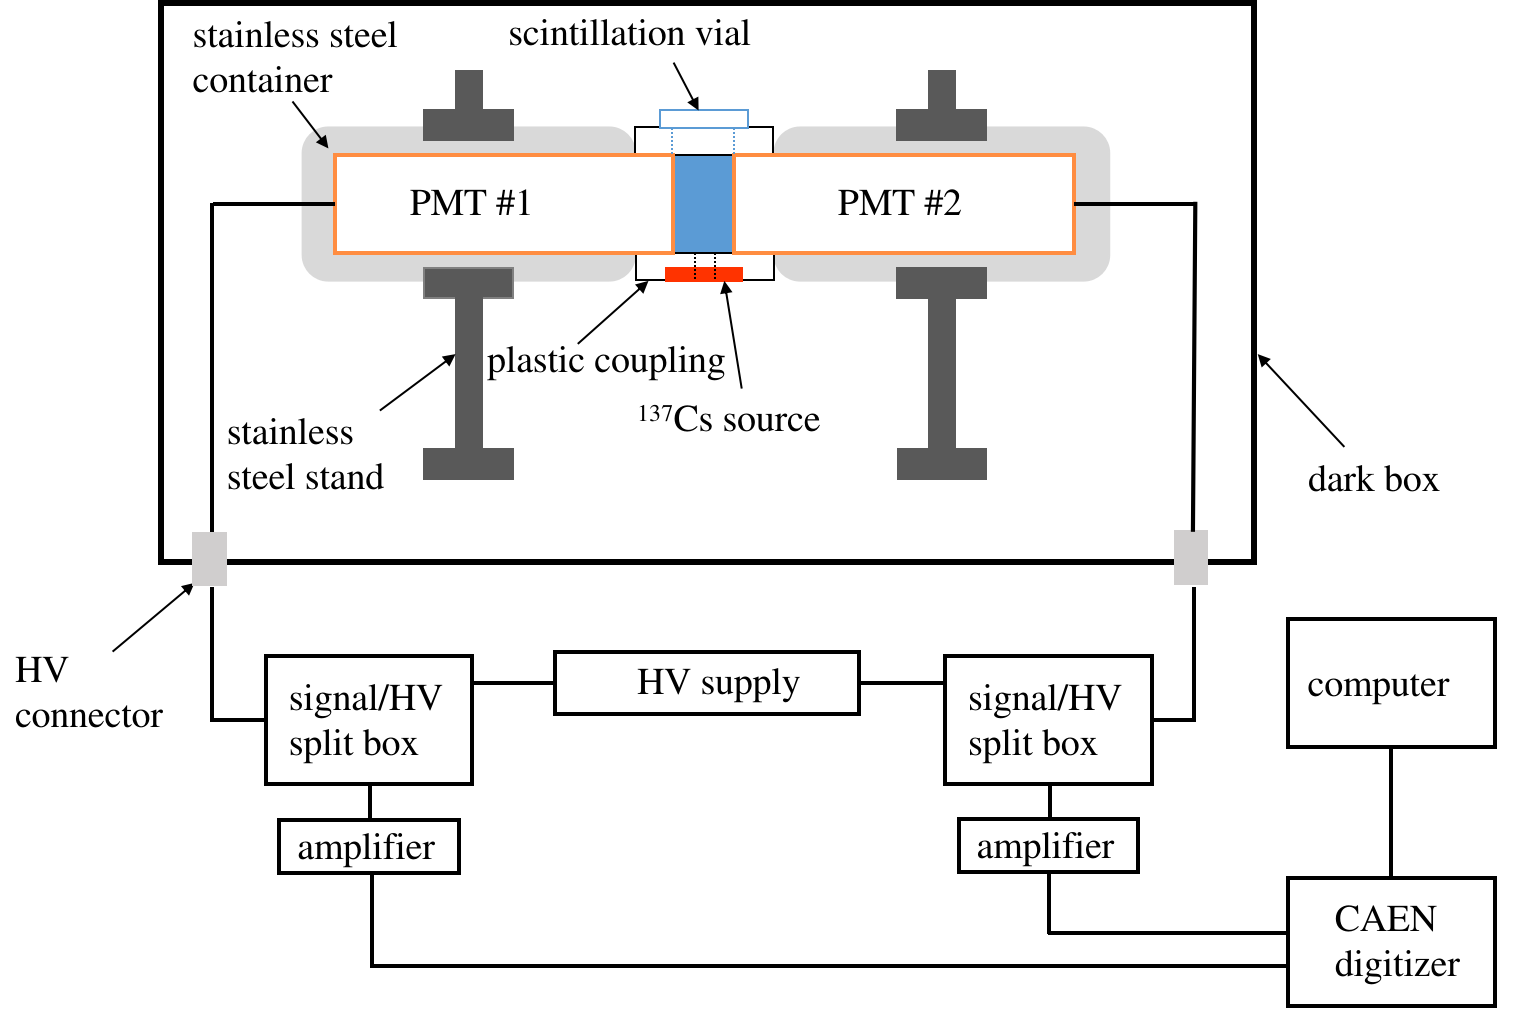
\includegraphics[width=10cm]{teLSsetup.png}
	\caption[A diagram shows the light yield measurement setup.]{A diagram shows the light yield measurement setup. See the text for details.}
	\label{teLSsetup}
\end{figure}

Fig.~\ref{teLSsetup} shows a diagram of the whole measurement setup. The plastic piece held the radioactive source and the scintillation vial. It also aligned two PMTs to face the scintillation vial from each side. The piece can shield lights from outside as well. These setups were placed in a dark box to prevent the lights from the lab. Two RG59/U-type high voltage (HV) cables connected the PMTs to an HV supply outside the dark box. The HV cables were connected to two signal/HV split boxes to separate the HV current and electrical signals. Due to the resistor of the split box, the HV supply was set to 2200 Volts (V) for the PMT operation, while the operation voltage suggested by the Hamamatsu is 1800 V. 

The signal cables from the split box were connected to a two-channel Hewlett Packard (HP) amplifier. This amplifier inverted the signals and amplified them by 26 dB. The amplified signals were then input into a two-channel digitizer. The digitizer recorded the data and sent them to a desktop computer.

To obtain and analyze the data, we used a desktop Waveform Digitizer, the DT5751 module provided by the Costruzioni Apparecchiature Elettroniche Nucleari (CAEN). Running at a digital pulse processing mode, the module records the digitized PMT waveforms with a data-taking rate of 1 GHz for each channel\cite{caen}.

This module was controlled by the \texttt{CoMPASS} software provided by CAEN. The software set up the threshold and trigger parameters. Once the triggered event passed the threshold, the software recorded event time, trigger flag, and waveform histograms from the two channels. By integrating the waveforms, the energy of a triggered event was calculated\cite{compass}.

Each channel recorded the signals from each PMT individually. With the two-PMT setup, we applied coincidence time mode measurements. In the coincidence mode, a coincidence time window between two channels was set to 48 ns. For a certain event, the \texttt{CoMPASS} software compares the event time difference between two channels and only records it if the event time difference is less than 48 ns. A smaller window of 10 ns was further applied for analysis.

\subsubsection{Measurement}

The liquid scintillator samples we have measured are LAB-PPO, TeDDA, and TeSOP. The unloaded LAB-PPO sample served as a standard candle. 

A Cesium-137 (\isotope[137]{Cs}) radioactive source was always placed at the bottom of the scintillation vials.
The source was made by Radiochemical Centre Amersham. The radioactivity measured on 1st April 1974 was $11.09~microcurie(\mu Ci)$, with an accuracy of $3.7\%$. The activity was expected to be 
$11.09\times ({\frac{1}{2}})^{\frac{46}{30.08}}=3.84~\mu Ci$ in 2020, considering a half-life of 30.08 years for the $^{137}$Cs\cite{nndc}.

The $^{137}$Cs isotope has a 85.10\% chance to emit 0.661 MeV $\gamma$-rays\cite{nndc}. These $\gamma$-rays can travel into the liquid scintillator samples in the vial, interact with the samples and create scintillation photon.

For each sample, measurements were taken for a one-minute time duration. Waveforms from the PMT photo-current signals were digitized in a 252 ns time window. Shown in Fig.~\ref{teLSwaveform} is a typical waveform caused by $\gamma$ rays interacted with the LAB-PPO sample. The p.e. signals triggered PMT pulses, and the pulses were digitized as waveforms. For each waveform, the digitizer firmware dynamically calculated the baseline as the mean value of 256 data points inside a moving time window of 252 ns. A threshold was set as 100 units above the baseline. The data point on the 90\% leading edge of the pulse was taken as the trigger time ($t_{trigger}$) tag.
From this $t_{trigger}$ tag, in the following 80-ns window, the digitizer did not calculate another trigger to avoid introducing another pulse (trigger hold-off). Also, from the $t_{trigger}$ tag, a pre-gate of 8 ns was set. The waveform was integrated into the time gate of $[t_{trigger}-8, t_{trigger}+72]$ ns. This gives the integrated charge, which was calculated as an A/D converter (ADC) channel number. If the measurement system can be calibrated, the ADC channel number can be exactly converted into the energy of the particle interaction. Since here we only interested in the photon numbers, we used the ADC channel as the energy. Once the pulse in the waveform passed the threshold and a triggered time tag can be found, the digitizer considered it as a triggered event. A time flow started when the measurement began. Timestamps were recorded as event time when the triggered event happened. The waveform was recorded, and the ADC channel number (energy) of this event was calculated.

\begin{figure}[htbp]
	\centering	
	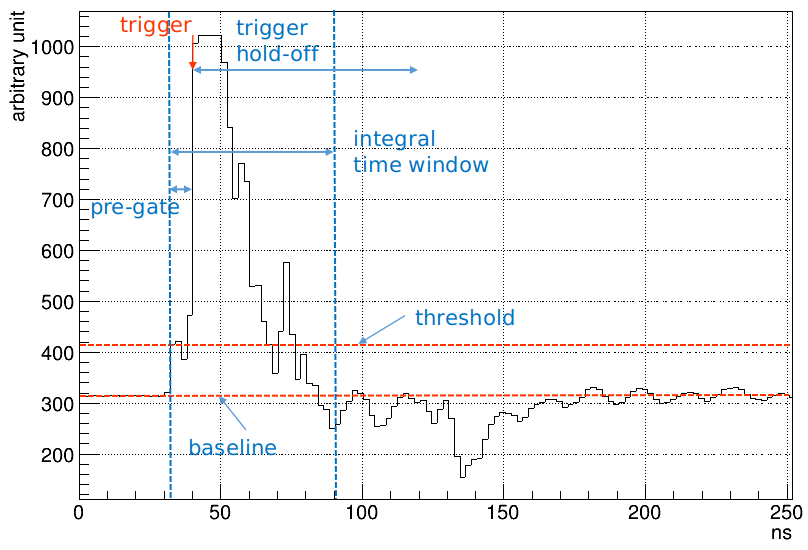
\includegraphics[width=8cm]{teLS_waveform.png}
	\caption[A typical triggered waveform.]{A typical waveform triggered by scintillation photons from $^{137}$Cs $\gamma$-rays interaction with LAB-PPO sample.}
	\label{teLSwaveform}
\end{figure}

In a coincidence time measurement, the event times of the events recorded by each of the two PMTs were compared. If the event time differences between two events from each PMTs were too long, these events were considered random noises rather than the physics events and were not recorded. We optimized a coincidence time cut as 40 ns and set that cut during the digitizer data-taking. 

\begin{figure}[htbp]
	\centering	
	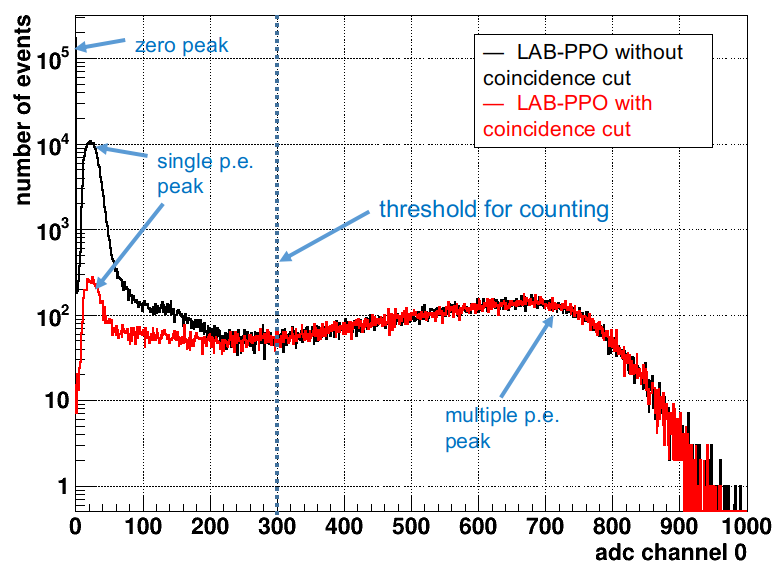
\includegraphics[width=10cm]{TeLScoinCut.png}
	\caption[Measured LAB-PPO energy spectrum with and without coincidence cut]{Measured LAB-PPO energy spectrum with and without coincidence cut on the ADC channel 0. A threshold for counting is set by comparing the two spectrum.}
	\label{teLScoinCut}
\end{figure}

Fig.~\ref{teLScoinCut} shows the measured LAB-PPO energy spectrum with and without coincidence time cut ($10~ns$) on the ADC channel 0.  Without the coincidence time cut, there is a zero peak caused by the pulses from random electronic noises or fluctuations of the digitized waveforms. The peak on the left is the single p.e. peak. It is mainly caused by some light sources which are weak enough that the photons only strike out at most one single p.e. inside the PMT\cite{leo2012techniques}.  The peak on the right is the multiple p.e. peak, in our case, which is mainly caused by some scintillation photons produced by the γ-ray interacting with the LAB-PPO. In the coincidence time measurement mode, it only records the photons detected by the two PMTs almost simultaneously. Therefore, the zero peaks are removed while the single p.e. peak is suppressed. The multiple p.e. peak is consistent with the non-coincidence measurement. A threshold in energy can be set to count only the scintillation photons emitted from LAB-PPO. 

\begin{figure}[htbp]
	\centering	
	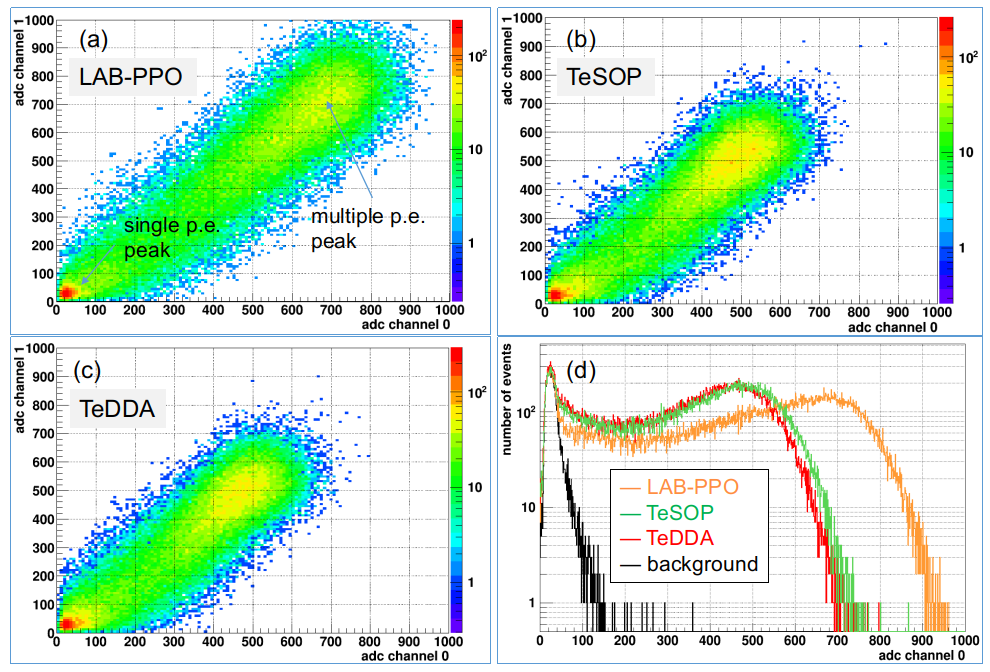
\includegraphics[width=14cm]{TeLS_2Denergy.png}
	\caption[The 2D energy spectrum of the counting measurements.]{The 2D energy spectrum of the counting measurements of LAB-PPO (a), TeSOP (b), and TeDDA (c) samples, projected the 2D plots into one channel (d). The single photo-electron (p.e.) peak is mainly caused by backgrounds while the multiple p.e. peak is from scintillation photons.}
	\label{teLSresults}
\end{figure}

Fig.~\ref{teLSresults} (a) shows the result of a one-minute measurement for the LAB-PPO sample. The data points in the 2D plot represent the triggered event fall in certain ADC channel numbers in each channel. A 10 ns coincidence window cut was applied to cut down noise, single p.e., and background events. The events in the 0 ADC channel, which represent noises, were totally cut off after applying the coincidence. Fig.~\ref{teLSresults} (b) and (c) show the results of the TeSOP and TeDDA samples respectively. Compared to the LAB-PPO sample, a shift of the multiple p.e. peak due to the different light yields can be observed clearly.

The 2D plots were projected onto a single channel, as shown in 
Fig.~\ref{teLSresults} (d). We used an empty vial and let $\gamma$-rays from $^{137}$Cs source passed through it as a background run (without the coincidence cut). This is to verify the single p.e. peak and noise region, shown as the black background spectrum.

From this plot, the single p.e. peaks for all the samples and the background match together. The multiple p.e. peaks indicate the different light yields of the scintillator samples. Here we can see the multiple p.e. peak of the LAB-PPO occupies the largest ADC channel number, while the channels of TeSOP are slightly larger than the TeDDA. 

To quantify the light yield differences between different samples, an analysis method of charge weighted photon number has been applied as the following:

First, from the energy spectrum, the single p.e. peak was fitted with an asymmetric Gaussian function (as $f_{asym}$ in \ref{eq:asyGaus}), as shown in Fig.~\ref{fitSinglePE}. The mean value of the asymmetric Gaussian ($p_0$) represents the ADC channel number corresponding to the single p.e. peak for the weighting. 

\begin{equation}\label{eq:asyGaus}
f_{asym}=c\cdot e^{-\frac{1}{2}(\frac{x-\mu}{\sigma})^2}\cdot Erfc(\xi),
\end{equation}
where $\xi=-\frac{\alpha(x-\mu)}{\sqrt 2\sigma},p_0=\mu,p_1=\sigma,p_2=\alpha, p_3=c$.

Then for the multiple p.e. region, weighting (dividing) the counts of the event in each channel with the single p.e. ADC channel number to calculate the total number of the photons.

\begin{figure}[htbp]
	\centering	
	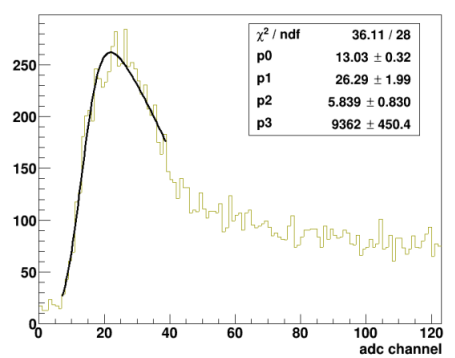
\includegraphics[width=6cm]{fitSinglePE.png}
	\caption[The single p.e. peak fitted with an asymmetric Gaussian function.]{The single p.e. peak is fitted with an asymmetric Gaussian function ($f_{asym}$) to obtain the ADC channel for weighting. The mean value of p0 is used as the adc channel relative to a single p.e. peak.}
	\label{fitSinglePE}
\end{figure}

To define the multiple p.e. region for the counting, the spectrum projected on each channel with and without coincidence cut are compared to define a threshold of the ADC channel for counting. By integrating from this threshold, the total numbers of events between two spectrum are close to each other. From two channels, we get two thresholds and then define a box cut in the 2D coincidence plot. We weights the events in the box to obtain the total number of photons. Fig.~ 16 and Fig.~ 19 show the case of the LAB-PPO sample.
\begin{figure}[htbp]
	\centering	
	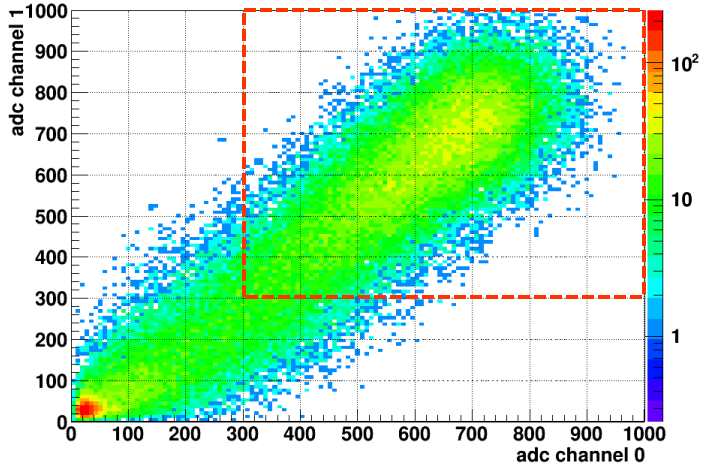
\includegraphics[width=6cm]{TeLS_2DboxCut.png}
	\caption[Two dimensional spectrum of LAB-PPO sample with coincidence cut.]{Two dimensional spectrum of LAB-PPO sample with coincidence cut. A box cut is defined for multiple PE counting.}
	\label{2DboxCut}
\end{figure}

Two dimensional spectrum of LAB-PPO with coincidence cut is shown in Fig.~\ref{2DboxCut}. A box cut is defined for multiple PE counting. 

Once the total number of photons for a certain sample is counted, we can calculate its ratio to the LAB-PPO sample to obtain the relative light yield.

\subsubsection{Results}
\begin{table}[ht]
	\centering
	\caption{\label{lightyield1} Number of photons calculated by Charge weighted photon number method.}
	\centering	
	\begin{tabular*}{100mm}{c@{\extracolsep{\fill}}cccc}
		\toprule 
		Sample & Number of photons ($\times 10^6$) & RLY\\
		\midrule
		LAB-PPO& 2.0811 & 1\\
		TeDDA& 1.2652 & 	0.61 \\
		TeSOP& 1.3976 & 0.67\\
		\bottomrule	
	\end{tabular*}
\end{table}

Table.~\ref{lightyield1} shows the number of photons calculated by the charge weighted photon number method.

Here we quantify the relative light yields of our samples. The light yield of the $0.5\%$ Te by SOP synthesis procedure (TeSOP) is $0.61$ and the one of the $0.5\%$ Te by DDA procedure is 0.67. The light yield of TeSOP is slightly larger than the TeDDA. In \cite{biller2017new}, a relative light yield of $\sim 0.65$ was reported.

\section{Electronics}
In this section, the SNO+ electronics system is introduced. The system includes the trigger and readout systems. As mentioned in \ref{sect:overview}, the PMTs as photon sensors are the basic detection elements for the SNO+ detector. The signals from the PMTs are sent to the SNO+ electronics system, which records the PMT time and charges information and then transfers the digitized data to offsite computing systems for data analysis. These steps are detailed in the following.

The photons created from particle interactions in the detector propagate to the PMT sphere and may hit a certain PMT and strike on its photo-cathode, which is a thin cesium bialkali film coated on the inner surface of PMT glass. The photocathode then produces a photo-electron (p.e.) through a photoelectric effect. The photocathode is set at ground voltage while the anode is at a high voltage ranging from $+1700$ to $+2100~V$ \cite{boger2000sudbury,dunger2018topological}. This forms electric fields inside the PMT. The p.e. is accelerated and focused by the electric field in the PMT and goes through the volume which is under vacuum until it reaches the region of a series of secondary emission electrodes, called dynodes. When the p.e. transfers its energy to the materials in dynodes, a number of secondary electrons escape and form a measurable current which is collected by a custom-made operating circuit (called ``PMT base'') at the anode\cite{hamamatsu2018photomultiplier}.

The anode pulse produced from the PMT travels along 35 m-long RG59/U type coaxial cable (with a resistance of 75 $\Omega$) to the front-end electronics which are set up on the deck above the detector. The coaxial cable also carries the high-voltage\cite{boger2000sudbury}. 

To tackle with more than 9000 PMTs in the SNO+ detector, the coaxial cables connected to each PMTs are grouped into bundles. Each bundle is connected to a Paddle Card, which are linked to a PMT Interface Card (PMTIC). The PMTIC supplies high voltages and receives signals from the PMTs. 32 channels (for 32 PMTs) in the PMTIC are plugged into a Front End Card (FEC) that processes, digitizes, and stores PMT signals. 19 crates tackle 9728 PMT channels in total, of which 32 channels are reserved for calibration inputs and labeled as FEC Diagnose (FECD) channels. These FECD channels are mainly used to tag calibration events. The triggered PMTs can be labeled by the logical channel number (lcn) using the map of the PMT to the crates and cards\cite{snop_jinst,stringer2019sensitivity}:
\begin{equation}
lcn = 512 \times crate + 32 \times FEC + channel
\end{equation}
%9605 are actually used

A 10 MHz and a 50 MHz clocks are used to record the time of the triggered event. The universal time of the triggered event is calculated as the time elapsed from a predefined $T_{zero}$, the midnight of January 1, 2010 (GMT) to the moment when the event happens. A 10 MHz clock used for counting the absolute time started at $T_{zero}$. It has a 53 bit register and can run for 28.5 years. Its accuracy is maintained by a GPS system. The 50 MHz clock gives more accurate timing. It limits the best time resolution of the GT to 20 ns. This clock has a 43 bit register and rolls over every 2.04 days. The relative time between the events can be used for analyzing specific physics processes, such as radioactive decays\cite{rattime,stringer2019sensitivity}. 

The recorded hit information of the triggered event, including the time and charge information of hit PMTs and the trigger settings, are sent to a Crate Controller Card (XL3) in each crate. These cards were installed for SNO+ to handle higher data transfer rates compared to SNO, with a max rate of 14 MB/s, which is equivalent to approximately 2 million hits per second\cite{bonventre2014neutron}. They read out the recorded data and wrap them as ethernet packets and send them to the Data Acquisition System (DAQ) and Event Builder system\cite{walker2016study}. The Event Builder system writes information into event records based on their GT identification number (GTID) and saves them on storage disk\cite{snop_jinst}. These raw data are written to the disc and are further processed into ROOT format by high-performance computing clusters.

As a summary, the SNO+ electronic system can measure signals with a nanosecond-level timing resolution and a single-photon level charge resolution. It can handle an event rate of several kHz and even much higher rates for cases such as the burst events from a galactic supernova\cite{snop_jinst}.

\section{Calibration}\label{sect:calibr}
Calibration sources with known physics parameters help to understand the detector response to the events and to make accurate measurements.

Two kinds of calibration sources are used by SNO+: (1) the optical sources to measure the \emph{in-situ} optical properties of the detector media and to calibrate the PMTs; and (2) the radioactive sources to test the detector energy responses, check the performance of event reconstruction algorithms for reconstructing event position, direction and energy and then determine their systematic uncertainties. Various types of radioactive sources producing different types of particles ($\beta,\gamma$ particles or neutrons) with different energies can also help to test the analysis tools for particle identifications.

The deployment of calibration sources at different positions in the detector can help to understand the asymmetries in the detector responses. The detector geometry is not perfectly symmetric, due to the presence of the AV neck, ropes, gaps between the PMTs, and the difference in individual PMTs\cite{snop_jinst}. 

The scan of the sources is realized through a source manipulator system (SMS)

umbilical vertical and side ropes

See Fig.~\ref{sms}.

 in the PSUP and differences    

All the calibration sources have been designed to meet the radiopurity required by SNO+ and their materials are compatible with the detection media\cite{snop_jinst}.


A Universal Interface (UI) connects the AV and the SMS. It is a sealed glove
box above the AV neck in a clean room set on the SNO+ deck.


reduce the radio contamination in the detector

\begin{figure}[!htb]
	\centering
	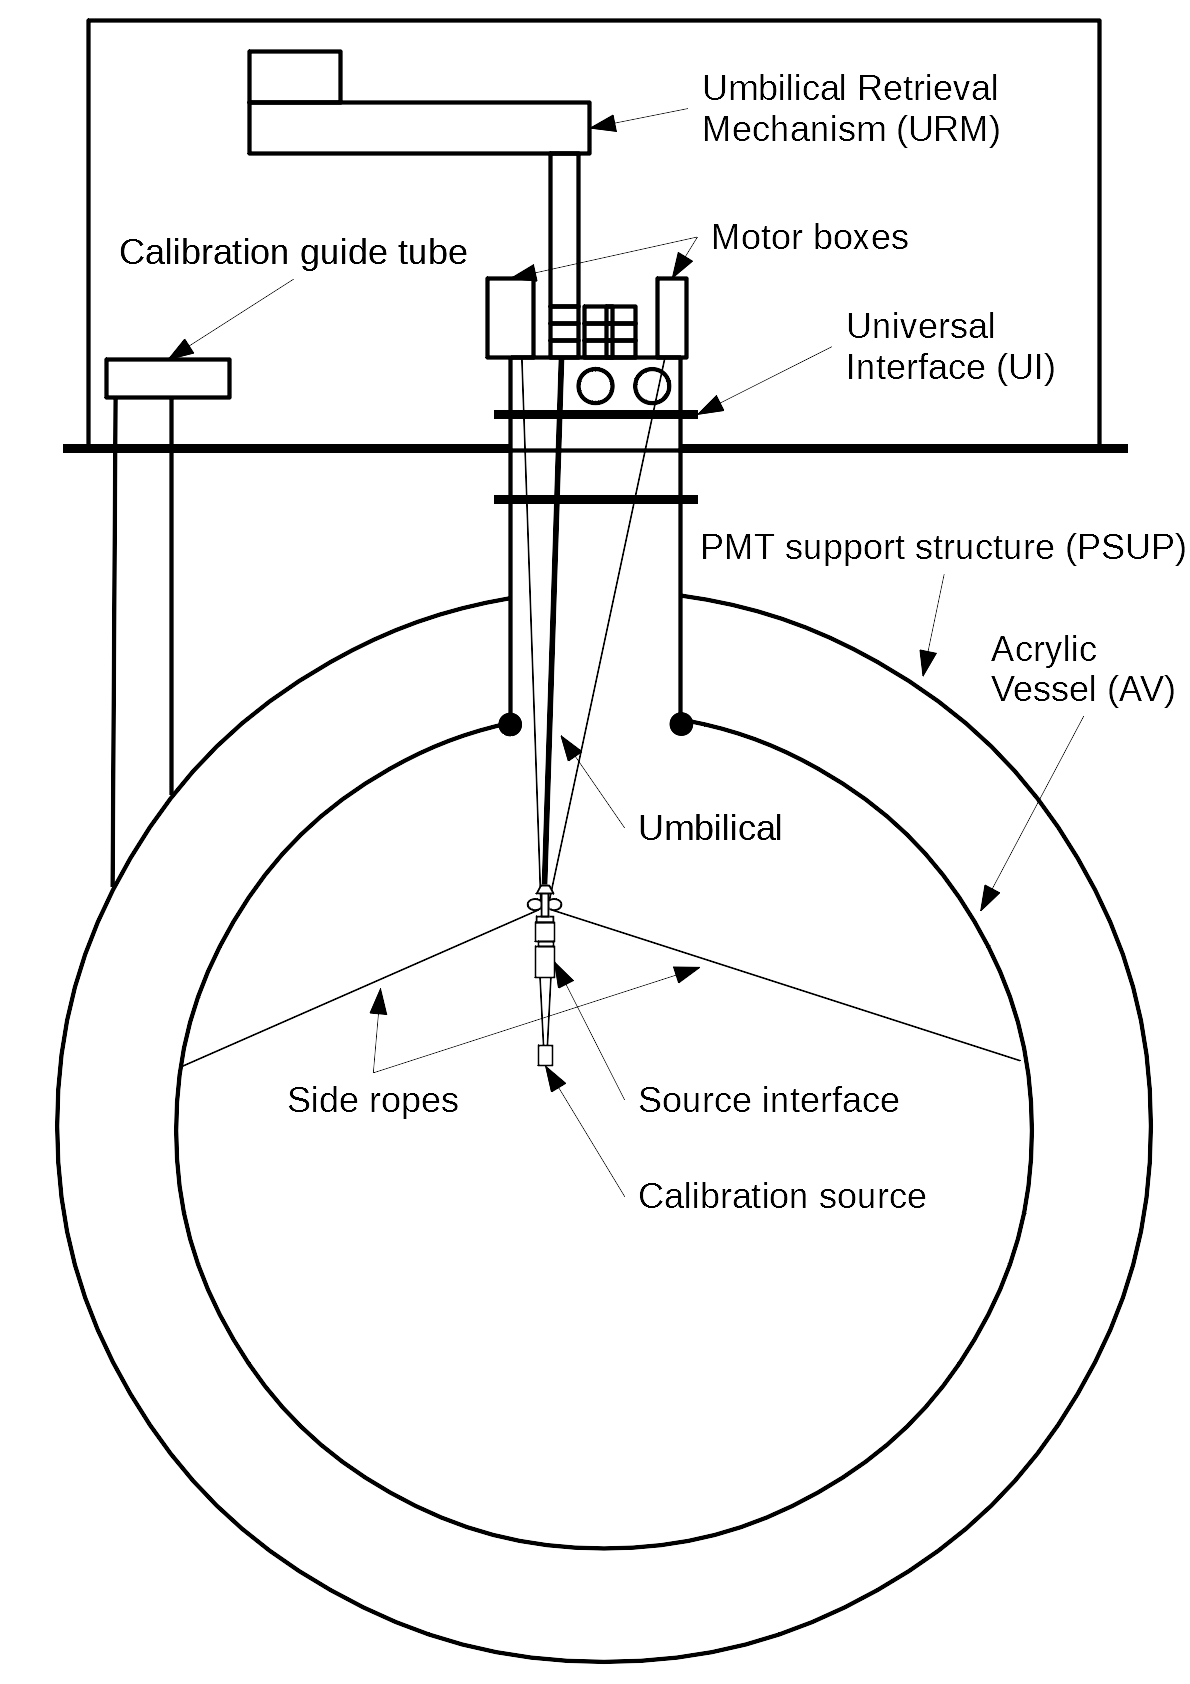
\includegraphics[width=8cm]{SMS.png}
	\caption{The SNO+ Source Manipulator System, taken from Ref.~\cite{snop_jinst}.}
	\label{sms}
\end{figure}

In addition, to measure the position of the calibration source deployed in the detector, six underwater cameras were mounted on the PSUP and work as a camera system to take photographs and then triangulate the source location. An accuracy of several centimeters is achieved. This system is also used to monitor the physical state of the detector, such as the offset of the AV center with respect to the PSUP, the movement of the rope net, the height of the water-scintillator interface during the partial-fill, etc\cite{singh2020underwater,snop_jinst}.

\subsection{Optical Calibration Sources}
The optical calibration sources are used to calibrate the PMT response and to measure the optical properties of the detector media. The optical sources mainly include a light diffusing sphere (called ``laserball", LB), as well as the Embedded Light-emitting diode (LED)/Laser Light Injection Entity (ELLIE)\cite{snop_jinst}.

The laserball injects lights from a nitrogen dye laser to a glass bubble.
\cite{anderson2021optical}.
fast pulsing LED or lasers
measures optical properties and parameters of describing the detector optical model,

, such as scattering, attenuation of the detector materials, the response of PMTs, angular and wavelength dependent wavelength dependent absorption and the optical degradation.

Optical calibration \emph{in-situ}

various dyes provide different peak wavelengths of the laser light, mainly at 365, 385, 420, 450 and 500 nm.

Due to the requirements of very low radioactive background levels for SNO+, frequent deployments of calibration sources inside the AV are needed to be avoided. To conduct weekly calibrations of the PMTs, the ELLIE system was developed by SNO+. It uses fast pulsing light injection devices which were mounted on the PSUP at fixed positions, covering all inward facing PMTs. The ELLIE system consists of three modules: (1) the timing module (TELLIE), which utilizes LED for calibrating the PMT hit-time and gains; (2) the scattering module (SMELLIE), which uses laser light to measure the Rayleigh scattering length and scattering angle of the detector media; (3) the attenuation module (AMELLIE), which is used to monitor the relative changes in attenuation lengths of detection media\cite{snop_jinst,jones2011background,walker2016study,dunger2018topological}.

\subsection{Radioactive Calibration Sources}
\subsubsection{The $^{16}$N Calibration Source}\label{n16_description}
The $^{16}$N calibration source is one of the radioactive sources. This source is inherit from the SNO experiment and has been well-understood\cite{dragowsky1999sudbury,dragowsky200216n,hamer2001energy}.   

Since the $^{16}$N isotope has a short half-life of $7.13~s$, it must be produced on-site during the calibration runs. A commercial deuterium-tritium (DT) generator was installed in SNOLAB to produce neutrons through the reaction: $D+T\to n+^{4}$He; then the produced 14-MeV neutrons interact with the CO$_2$ gas streaming through the small diameter capillary tubing and produce the $^{16}$N isotopes via the $(n,p)$ reaction: $n+^{16}$O$\to^{16}$N$+p$. These $^{16}$N isotopes are transferred into the cavity or the detector by the CO$_2$ gas tubing\cite{dragowsky200216n}.  

The $^{16}$N isotope mainly decays through $\beta$-decay process: $^{16}$N$\to ^{16}$O$+e^-+\bar{\nu}_e$. It has a 66.2\% chance to emit an electron with $E_{end~point}=4.29$ MeV and a 22.8\% chance to an electron with $E_{end~point}=10.42$ MeV; while the resulting $^{16}$O deexcites and produces a cascade of $\gamma$'s. There are mainly 6.13-MeV $\gamma$ with an intensity of 67.0\% and 7.12-MeV $\gamma$ with an intensity of 4.9\%. The intensities of the $\gamma$ particles with other energies are all below 1\%\cite{nndc}. A simplified decay scheme is shown in Fig.~\ref{n16decay}.

\begin{figure}[!htb]
	\centering
	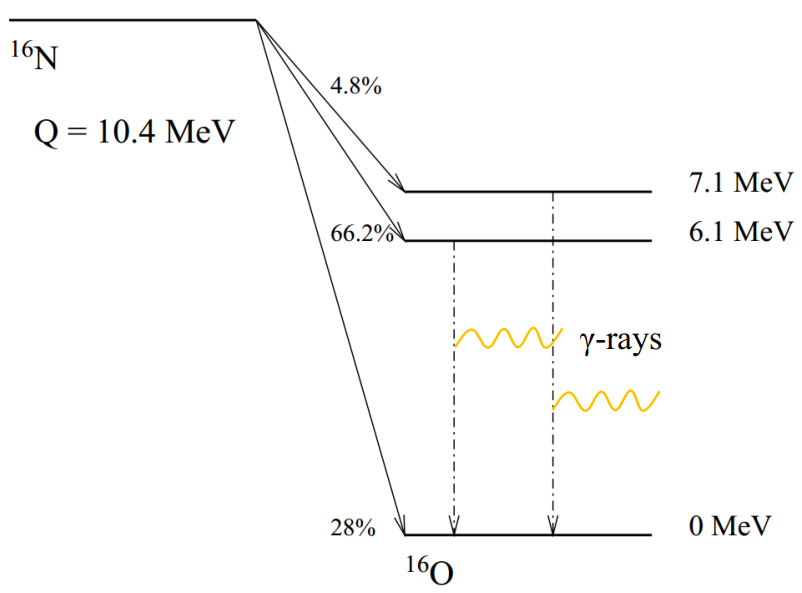
\includegraphics[width=6cm]{n16_decay.png}
	\caption[$^{16}$N main decay scheme]{$^{16}$N main decay scheme, modified from Ref.~\cite{dragowsky200216n}.}
	\label{n16decay}
\end{figure}

Fig.~\ref{n16pic} shows the geometry of the $^{16}$N source chamber. The chamber is a stainless steel cylinder mainly containing a small PMT and a gas decay chamber. The chamber was designed to confine the electrons from $^{16}$N decay within the chamber and let them be detected by the PMT inside\cite{dragowsky1999sudbury}.

%to ensure a high fraction of the $\gamma$-rays 

%lighthouse where the liquid in the scintillator volume (for example, pure water in the water phase) is free to enter.
%tagged by a small PMT inside

%A polyethelene bumper cone is at the bottom of the source.

%gas capillary tube 


\begin{figure}[!htb]
	\centering
	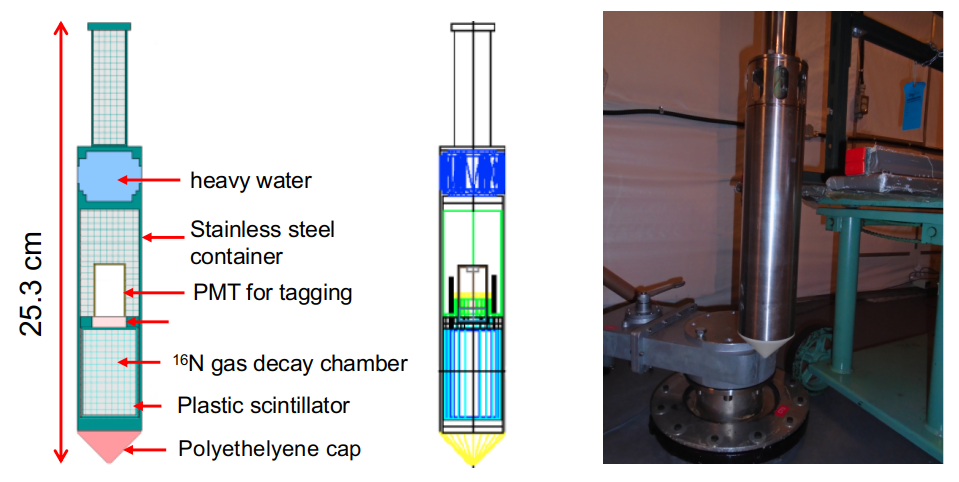
\includegraphics[width=10cm]{n16geom.png}
	\caption[$^{16}$N calibration source geometry.]{$^{16}$N calibration source geometry. Left: a detailed diagram of $^{16}$N source geometry, modified from Refs.~\cite{maclellan2009energy,matt_deployedsource}; middle: source geometry implemented in RAT, modified from Ref.~\cite{n16geom_zach}; right: a picture of the $^{16}$N source, taken from \cite{n16pic}.}
	\label{n16pic}
\end{figure}

%The $^{16}$N source $^{3}$H$(p,\gamma)^{4}$He reaction.

A detailed study of using the $^{16}$N source for testing and estimating the reconstruction uncertainties will be shown in \ref{sect:n16_water}.

\subsubsection{The Americium Beryllium Calibration Source}\label{sect:AmBesource}
Also being inherited from the SNO collaboration, the americium-beryllium (AmBe) source 
is used to produce neutrons and a 4.4-MeV $\gamma$ with a of 59\%. The $\alpha$-emitter $^{241}$Am  


  9Be target

the neutrons are expected to be captured and it emits 2.2-MeV delayed $\gamma$s. 
\begin{equation}
\begin{split}
\alpha + \isotope[9]{Be} \to \isotope[12]{C} + n (40.9\%),\\
\alpha + \isotope[9]{Be} \to \isotope[12]{C}^* + n (59.1\%),\\
\isotope[12]{C}^* \to \isotope[12]{C} + \gamma (4.4~MeV),\\
\end{split}
\end{equation}

The 9Be nucleus then produces a 12C nucleus through neutron emission. If the 12C nucleus is produced
in an excited state, it will de-excite by emitting at least one γ-ray. The γ radiation from this reaction is
predominantly 4.4 MeV, and occurs whenever the 12C is not formed in the ground state. Depending on the
form and setup of the source, these γ-rays accompany ($59.1\pm 1.5$)\% of all neutrons 

\subsubsection{Other Calibration Sources}

New calibration sources are being developed to calibrate the energy scale in the scintillator and tellurium-loading phases, especially for the energy region of interest (ROI) in the $0\nu\beta\beta$ study. They are the $^{46}$Sc tagged source with a PMT and three additional untagged $\gamma$ sources: $^{48}$Sc, $^{137}$Cs and $^{57}$Co\cite{snop_jinst}. Among them, the isotopes of $^{48}$Sc ($T_{1/2}$=43.67 hours, 100\% $\beta^-$ decay) and $^{137}$Cs ($T_{1/2}$=30.1 years, 100\% $\beta^-$ decay) can provide both the $\beta^-$ and $\gamma$ particles while the $^{57}$Co  ($T_{1/2}$=271.74 days, 100\% electron capture) only emits $\gamma$s. They can provide $\gamma$s with energies ranging from 14 keV ($^{57}$Co) to 1310 keV ($^{48}$Sc) and $\beta^-$ particles with energies ranging from 480 keV ($^{48}$Sc) to 1176 keV ($^{137}$Cs)\cite{nndc}.

\section{Monte Carlo Simulation and RAT Software}\label{sect:rat}
The SNO+ collaboration uses a software package called the Reactor Analysis Tool (\texttt{RAT}) for Monte Carlo simulation as well as event-based analysis offline and online. To accomplish these two tasks, \texttt{RAT} integrates the \texttt{Geant4} simulation toolkit\cite{agostinelli2003geant4} and ROOT data analysis framework\cite{brunroot} for processing and analyzing data. This feature makes it easy to analyze Monte Carlo-generated events and real data in a same framework and data structure.

The software was originally developed by Stan Seibert from the Braidwood Collaboration to simulate a generic KamLAND-like detector\cite{ratManual}. A simulation package called Generic Liquid Scintillator \texttt{Geant4} simulation (\texttt{GLG4sim}) was developed and implemented in \texttt{RAT}\cite{horton2006introduction}. It simulates the scintillation physics processes, the generations of scintillation photons and also the propagation, reflections, refraction, scattering ans absorption of optical photons\cite{dunger2018topological}.

The SNO+ version of \texttt{RAT} links the existing \texttt{ROOT}, \texttt{Geant4} and \texttt{GLG4sim} packages to minimize the code duplication. The SNO+ \texttt{RAT} is being developed by the whole collaboration and evolves with the experiment progress to precisely simulate the SNO+ detector in different physics phases as well as applying multiple analysis tasks. The relative flexible code structure of \texttt{RAT} allows the user to introduce their own code into the simulation or analysis process\cite{ratManual}. It can be updated and optimized with the measured parameters from detector calibration; it can be added with more precise descriptions of the physics processes in the detector; it can also be introduced with more advanced analysis tools. The users can apply different analysis tasks, such as different reconstruction algorithms on the same events\cite{ratManual}. Therefore, different versions of \texttt{RAT} serving to different SNO+ physics phases may give different outputs. For the work in this thesis, multiple \texttt{RAT} versions were used, mainly the versions for the water phase and partial-fill phase. In this case, I will specify the \texttt{RAT} version when I discuss a specific analysis.

\texttt{RAT} is also used by other astroparticle physics experiments, such as the dark matter experiment DEAP/CLEAN\cite{caldwell2014simulation}. 